\documentclass[tikz,border=2pt]{standalone}
\usepackage{amsmath}
\usetikzlibrary{arrows.meta}
\newcommand{\angl}[1]{\overline{#1}\rvert}
\begin{document}
% Three unit payments at v = 0.9: the annuity-due pays at 0,1,2 (value 1 + 0.9 + 0.81 = 2.71),
% the annuity-immediate pays at 1,2,3 (value 0.9 + 0.81 + 0.729 = 2.439 = 0.9 x 2.71).
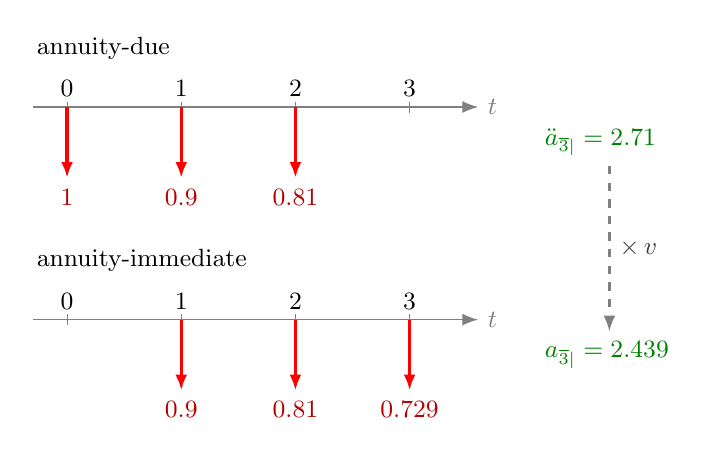
\begin{tikzpicture}[font=\small, >={Latex[length=2mm]}, x=1.45cm, y=1cm]
  \foreach \row/\yy/\first/\name/\val in {due/0/0/{annuity-due}/{$\ddot a_{\angl{3}}=2.71$},imm/-2.7/1/{annuity-immediate}/{$a_{\angl{3}}=2.439$}} {
    \begin{scope}[yshift=\yy cm]
      \node[anchor=west] at (-0.35,0.75) {\name};
      \draw[gray, ->] (-0.3,0) -- (3.6,0) node[right] {$t$};
      \foreach \k in {0,...,3} {
        \draw[gray] (\k,-0.07) -- (\k,0.07);
        \node[above, inner sep=2pt] at (\k,0.05) {$\k$};
      }
      \node[green!50!black, anchor=west] at (4.1,-0.45) {\val};
    \end{scope}
  }
  % payments (unit, downwards) with their present values
  \foreach \k/\pv in {0/{1},1/{0.9},2/{0.81}} {
    \draw[->, red, very thick] (\k,0) -- (\k,-0.9);
    \node[red!70!black, anchor=north] at (\k,-0.92) {$\pv$};
  }
  \begin{scope}[yshift=-2.7cm]
    \foreach \k/\pv in {1/{0.9},2/{0.81},3/{0.729}} {
      \draw[->, red, very thick] (\k,0) -- (\k,-0.9);
      \node[red!70!black, anchor=north] at (\k,-0.92) {$\pv$};
    }
  \end{scope}
  % shift by one year multiplies by v
  \draw[->, gray, thick, dashed] (4.75,-0.75) -- node[right, gray!50!black] {$\times\,v$} (4.75,-2.85);
\end{tikzpicture}
\end{document}
